\section{The Algebraic and Order Limit Theorems}
    \textbf{Definition 2.3.1.} A sequence $(x_n)$ is \textit{bounded} if there exists a number $M > 0$ such that $|x_n| \leq M$ for all $n \in \textbf{N}$.
    \newline \indent This means $[-M, M]$ contains every term in $(x_n)$
    \setcounter{theorem}{1}
    \begin{theorem}
        Every convergent sequence is bounded. 
    \end{theorem}
    \begin{proof}
        Assume $(x_n)$ converges to a limit $l$. So for any value of $\epsilon$, there exists an $N \in \textbf{N}$ such that if $n \geq N$, then $x_n$ is in the interval $(l - \epsilon, l + \epsilon)$, or 
        $$|x_n| < |l| + \epsilon$$
        for all $n \geq N$, for any value of $\epsilon$.
        \newline
        \begin{center}
            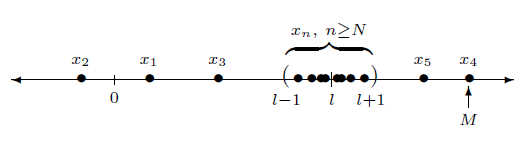
\includegraphics[width=250pt]{converges.png}
        \end{center}
        Since there are only a finite number of terms before $N$, we let
        \begin{equation*}
            M = max\{|x_1|, |x_2|, |x_3|, \dots, |x_{N-1}|, |l| + \epsilon\}
        \end{equation*}
        Then it follows that $|x_n| \leq M$ for all $n \in \textbf{N}$ as desired.
    \end{proof}
    \begin{theorem}[Algebraic Limit Theorem]
        Let $\lim a_n = a$, and $\lim b_n = b$. Then,
        \newline
        (i) $\lim(ca_n) = ca$, for all $c \in \textbf{R}$;
        \newline
        (ii) $\lim(a_n + b_n) = a + b$;
        \newline
        (iii) $\lim(a_nb_n) = ab$;
        \newline
        (iv) $\lim(a_n/b_n) = a/b$, provided $b \neq 0$;
    \end{theorem}
    \begin{proof}
        (i) Consider if $c \neq 0$. Let $\epsilon$ be some arbitrary positive number. We want to show that after some point in the sequence $(ca_n)$, 
            $$|ca_n - ca| < \epsilon$$
            Now,
            $$|ca_n - ca| = |c||a_n - a|$$
            Since $(a_n) \rightarrow a$, we can make $|a_n - a|$ as small as we want. So we choose an $N$ so
            $$|a_n - a| < \frac{\epsilon}{|c|}$$
            whenever $n \geq N$. Then, 
            $$|ca_n - ca| = |c||a_n - a| < |c|\frac{\epsilon}{|c|} = \epsilon$$
            The case $c = 0$ reduces to showing the constant sequence $(0, 0, 0, \dots)$ converges to 0. Let $\epsilon > 0$ be arbitrary. Then for any $N \in \textbf{N}$,
            $|ca_n - ca| < \epsilon$
            for all $n \geq \textbf{N}$ since $|0 - 0| = 0 < \epsilon$.
        \newline \indent
        (ii) Now, we are proving
            $$|(a_n + b_n) - (a + b)|$$
            can be made less than an arbitrary $\epsilon$. First, use the triangle inequality to say
            $$|(a_n + b_n) - (a + b)| = |(a_n - a) + (b_n - b)| \leq |a_n - a| + |b_n - b|$$
            Since $(a_n) \rightarrow a$ and $(b_n) \rightarrow b$, we know there exists an $N_1$ and $N_2$ such that 
            $$|a_n - a| < \frac{\epsilon}{2} \text{ whenever } n \geq N_1$$
            and
            $$|b_n - b| < \frac{\epsilon}{2} \text{ whenever } n \geq N_2$$
            Now, let $N = max\{N_1, N_2\}$ so that when $n \geq N$, then $n \geq N_1$ and $n \geq N_2$. So,
            \begin{align*}
                |(a_n + b_n) - (a + b)| = |(a_n - a) + (b_n - b)| \leq |a_n - a| + |b_n - b| \\
                < \frac{\epsilon}{2} + \frac{\epsilon}{2} = \epsilon
            \end{align*}
            for all $n \geq N$, as desired.
        \newline \indent
        (iii) To begin,
            \begin{align*}
                |a_nb_n - ab| = |a_nb_n - ab_n + ab_n - ab| \\
                \leq |a_nb_n - ab_n| + |ab_n - ab| \\
                = |b_n||a_n - a| + |a||b_n - b|
            \end{align*}
            Let $\epsilon > 0$ be arbitrary. For $|a||b_n - b|$, we can choose $N_1$ so that
            $$n \geq N_1 \text{ implies } |b_n - b| < \frac{1}{|a|}\frac{\epsilon}{2}$$
            as long as $a \neq 0$. This causes the right side to be less than $\frac{\epsilon}{2}$ Now for $|b_n||a_n - a|$, we know $|b_n| \leq M$ for some $M$ since it is bounded. So, 
            $$|b_n||a_n - a| \leq M|a_n - a|$$
            So we choose an $N_2$ so that
            $$|a_n - a| < \frac{1}{M}\frac{\epsilon}{2} \text{ whenever } n \geq N_2$$
            Now, pick $N = max\{N_1, N_2\}$, and observe that if $n \geq N$, then
            \begin{align*}
                |a_nb_n - ab| = |a_nb_n - ab_n + ab_n - ab| \\
                \leq |a_nb_n - ab_n| + |ab_n - ab| \\
                = |b_n||a_n - a| + |a||b_n - b| \\
                \leq M|a_n - a| + |a||b_n - b| \\
                < M(\frac{\epsilon}{M2}) + |a|(\frac{\epsilon}{|a|2}) = \epsilon
            \end{align*}
        (iv) This is proven by (iii) if we can prove that
            $$(b_n) \rightarrow b \text{ implies } (\frac{1}{b_n}) \rightarrow \frac{1}{b}$$
            whenever $b \neq 0$.
            $$|\frac{1}{b_n} - \frac{1}{b}| = \frac{|b - b_n|}{|b||b_n|}$$
            We can make $|b - b_n|$ as small as we want. To find a worst case estimate of $|b||b_n|$, we must find a lower bound greater than 0. Consider $\epsilon_0 = |b|/2$. Since $(b_n) \rightarrow b$, there exists an $N_1$ such that $|b_n - b| < |b|/2$ for all $n \geq N_1$. This implies $|b_n| > |b|/2 > 0$. 
            \newline \indent
            Next, choose $N_2$ so that $n \geq N$ implies
            $$|b_n - b| < \frac{\epsilon|b|^2}{2}$$
            Finally, set $N = max\{N_1, N_2\}$, then $n \geq N$ implies
            $$|\frac{1}{b_n} - \frac{1}{b}| = |b - b_n|\frac{1}{|b||b_n|} < \frac{\epsilon|b|^2}{2}\frac{1}{|b|\frac{|b|}{2}} = \epsilon$$
    \end{proof}
    \subsection*{Limits and Order}
        \begin{theorem}[Order Limit Theorem]
            Assume $\lim a_n = a$ and $\lim b_n = b$
            \newline
            (i) if $a_n \geq 0$ for all $n \in \textbf{N}$, then $a \geq 0$.
            \newline
            (ii) if $a_n \geq b_n$ for all $n \in \textbf{N}$, then $a \geq b$.
            \newline
            (iii) If there exists $c \in \textbf{R}$ for which $c \leq b_n$ for all $n \in \textbf{N}$, then $c \leq b$. And same for $a_n$ and $a$.
        \end{theorem}
        \begin{proof}
            (i) We prove this by contradiction. Assume $a < 0$. Then, consider a value of $\epsilon_0 = |a|$. The definition of convergence guarantees that we can find an $N$ such that $|a_n - a| < |a|$ for all $n \geq N$. This means that $|a_N - a| < |a|$, which implies $a_N < 0$, which contradicts that $a_N \geq 0$. We therefore conslude that $a \geq 0$.
            \newline
            (ii) The Algebraic Limit Theorem ensures that the sequence $(b_n - a_n)$ converges to $b - a$. Because $b_n - a_n \geq 0$, we can apply part (i) to get that $b - a \geq 0$.
            \newline
            (iii) Take $a_n = c$ (or $b_n = c$) for all $n \in \textbf{N}$, and apply (ii).
        \end{proof}
        In this theorem, we assumed things for all $n \in \textbf{N}$, but these properties hold true if these assumptions are true for all $n \geq N$, where $N$ is a finite natural number. If a property is of this form it is said to be \textit{eventually} true. Theorem 2.3.4, part (i), could be restated, "Convergent sequences that are eventually nonnegative converge to nonnegative limits."